\documentclass[10pt,conference,compsocconf]{IEEEtran}
\raggedbottom

\usepackage{hyperref}
\usepackage{graphicx}	% For figure environment
\usepackage{booktabs}
\usepackage{tabularx}
\usepackage{float}

\begin{document}
\title{Writing Scientific Papers and Software}

\author{
  Cheng Soon Ong\\
  \textit{Department of Computer Science, ETH Zurich, Switzerland}
}

\maketitle

\begin{abstract}

\end{abstract}

\section{Model and Methods}
\subsection{Data Processing}

Our initial dataset consists of 328,135 samples with 28,975 positive entries (~9\%), which indicate an important class imbalance. Additionally, the dataset contains identifiers, survey questions and body measurement
resulting in a very inhomogeneous feature space. We also note that some feature have dependencies (e.g. one questions depends on a positive answer to a previous question), some feature can contain entries with different scale
(e.g. height in meter or centimeter), and missing entries indicated by special codes defined in the BFRSS codebook. We thus proceed by implementing a data processing pipeline to prepare the data for training. \\

We decompose the processing of our training data into two phases. The first phase clean the features to ensure consistent
scale (e.g. weight in KG), replacing BRFSS codes with NAN or meaningful values, removing identifiers and highly incomplete data. We also decompose feature with a high percentage
of missing value into a pair of features which consists of a 0/1 categorical feature indicating the existence or not of the value and a feature containing the original magnitude. 

\begin{table}[H]
  \centering
  \caption{}
  \label{tab:cleaning}
  \footnotesize
  \setlength{\tabcolsep}{4pt}
  % no gap in the vertical lines at the horizontal rules
  \setlength{\aboverulesep}{0pt}
  \setlength{\belowrulesep}{0pt}
  \renewcommand{\arraystretch}{1.3}
  \newcommand{\step}[2]{#1\newline\hspace*{1em}\textit{e.g.\ #2}}
  \newcommand{\phase}[1]{\multicolumn{1}{@{}l|}{\textbf{#1}} & & & \\}
  \begin{tabularx}{\linewidth}{@{}>{\raggedright\arraybackslash}X|r|r|r@{}}
    \toprule
    Step & Change & Modified & Features \\
    \midrule
    Raw BRFSS features & & & 321 \\
    \phase{Cleaning}
    \step{``Don't know'' / ``refused'' codes $\rightarrow$ NaN}{PHYSHLTH: 77, 99 $\rightarrow$ NaN} & & 247 & 321 \\
    \step{``None'' / ``never'' codes $\rightarrow$ 0}{PHYSHLTH: 88 (no bad day) $\rightarrow$ 0} & & 32 & 321 \\
    \step{Units normalization}{ALCDAY5: 203 $\rightarrow$ 0.1/day} & & 19 & 321 \\
    \step{Identifiers}{\_LLCPWT, survey weight} & $-22$ & & 299 \\
    \step{Missing indicators ($> 5\%$ NaN)}{INCOME2\_missing = 1 if NaN} & $+222$ & & 521 \\
    \phase{Quality filters}
    \step{Constant (top value $\geq 99\%$)}{PVTRESD1, private residence} & $-8$ & & 513 \\
    \step{Incomplete ($> 99\%$ NaN)}{ASATTACK, asthma attack} & $-28$ & & 485 \\
    \step{Target leak}{HAREHAB1\_missing} & $-1$ & & 484 \\
    \bottomrule
  \end{tabularx}
\end{table}

As part of this process we identified a particularly high correlation to the output for the feature "HAREHAB1". After further inspection 
the feature is defined in the CDC codebook as follows.

\vspace{0.5em}
\begin{quote}
  \texttt{HAREHAB1}: \emph{``Following your heart attack, did you go to any kind of
  outpatient rehabilitation? This is sometimes called `rehab.'\,''}
\end{quote}
\vspace{0.5em}

It is clear that a patient that answers yes to this question had a heart attack, and thus we filter it out as well to avoid contamination. \\

The second phase builds the feature space before training. Note that aall the statistics used as filtering criterion have been computed on the training split only. 
We use one-hot encoding for k-value categorical feature because our linear model cannot use code as ordinal values and we clip outliers. We also
filter out duplicated feature using the correlation matrix, and we also remove feature that have almost no correlation with the output.  
Finally, we replace NAN with the training mean before normalizing each feature to be zero mean, unit variance.

\begin{table}[H]
  \centering
  \caption{}
  \label{tab:features}
  \footnotesize
  \setlength{\tabcolsep}{4pt}
  % no gap in the vertical lines at the horizontal rules
  \setlength{\aboverulesep}{0pt}
  \setlength{\belowrulesep}{0pt}
  \renewcommand{\arraystretch}{1.3}
  \newcommand{\step}[2]{#1\newline\hspace*{1em}\textit{e.g.\ #2}}
  \newcommand{\phase}[1]{\multicolumn{1}{@{}l|}{\textbf{#1}} & & & \\}
  \begin{tabularx}{\linewidth}{@{}>{\raggedright\arraybackslash}X|r|r|r@{}}
    \toprule
    Step & Change & Modified & Features \\
    \midrule
    Initial #Features & & & 484 \\
    \phase{Encoding}
    \step{One-hot encoding}{MARITAL $\rightarrow$ 6 dummies} & $+315$ & 36 & 799 \\
    \step{Outliers clipped - 1st / 99th percentiles}{\_BMI5, body mass index} & & 63 & 799 \\
    \phase{Selection}
    \step{feature - output correlation ($|\rho_y| < 0.01$)}{MARITAL\_4, separated} & $-296$ & & 503 \\
    \step{feature - feature ($|\rho| \geq 0.95$)}{EXEROFT2, $= $ PAFREQ2\_$\,/\,7$} & $-148$ & & 355 \\
    \phase{Scaling}
    \step{NaN $\rightarrow$ training mean}{INCOME2, income bracket} & & 171 & 355 \\
    \step{Standardization}{zero mean, unit variance} & & 355 & 355 \\
    Bias column & $+1$ & & 356 \\
    \bottomrule
  \end{tabularx}
\end{table}

We evaluate the effect of our processing pipeline on the data by plotting a heatmap of the feature's correlation matrix. TODO
\begin{figure}[t]
  \centering
  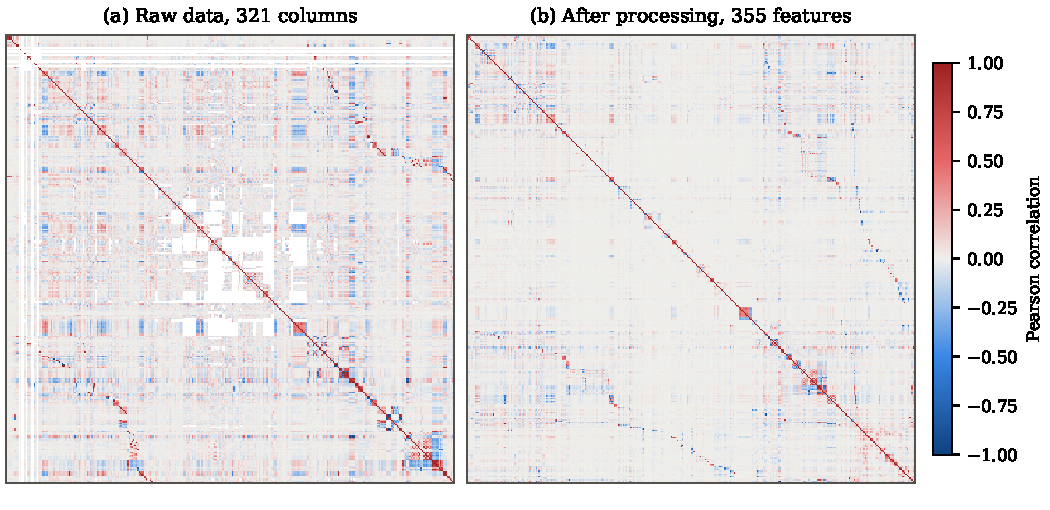
\includegraphics[width=\columnwidth]{correlation_heatmaps.pdf}
  \caption{Feature--feature Pearson correlation.}
  \label{fig:correlation}
\end{figure*}

\section{Model Selection}

\section{Evaluation}

\section{}

\section*{Acknowledgements}
The author thanks Christian Sigg for his careful reading and helpful
suggestions.

\bibliographystyle{IEEEtran}
\bibliography{literature}

\end{document}
